\documentclass[aspectratio=169,11pt]{beamer}
\usetheme{Madrid}
\usecolortheme{default}
\usefonttheme{professionalfonts}
\setbeamertemplate{navigation symbols}{}
\setbeamertemplate{footline}[frame number]
\setbeamertemplate{itemize items}[circle]
\setbeamertemplate{enumerate items}[default]
\usepackage[T1]{fontenc}
\usepackage[utf8]{inputenc}
\usepackage{lmodern}
\usepackage{amsmath,amssymb,bm}
\usepackage{booktabs}
\usepackage{multirow}
\usepackage{tikz}
\usetikzlibrary{arrows.meta,positioning,calc,fit,backgrounds,shapes.geometric}
\usepackage{xcolor}
\definecolor{accent}{RGB}{25,84,166}
\definecolor{softblue}{RGB}{235,242,252}
\definecolor{softgray}{RGB}{245,246,248}
\setbeamercolor{title}{fg=accent}
\setbeamercolor{frametitle}{fg=accent}
\setbeamercolor{structure}{fg=accent}
\setbeamercolor{block title}{bg=accent!12,fg=black}
\setbeamercolor{block body}{bg=softgray,fg=black}
\newcommand{\E}{\mathbb{E}}
\newcommand{\R}{\mathbb{R}}
\newcommand{\gp}{\mathcal{GP}}
\newcommand{\Normal}{\mathcal{N}}
\title{GP, GPSSM, and EnKF\\[2mm]\large How They Are Combined in EnVI}
\author{Based on the paper ``Gaussian Process State Space Models using Ensemble Kalman Filters''}
\date{}

\begin{document}

\begin{frame}[plain]
\vspace{0.3cm}
\begin{beamercolorbox}[wd=\textwidth,rounded=true,shadow=true,sep=0.55cm]{title}
  {\color{white}\LARGE\bfseries GP, GPSSM, and EnKF}\\[2mm]
  {\color{white}\large How They Are Combined in EnVI}
\end{beamercolorbox}

\vspace{0.6cm}
\begin{block}{Source}
Based on the paper \emph{Gaussian Process State Space Models using Ensemble Kalman Filters}.
\end{block}

\vspace{0.25cm}
\end{frame}

\begin{frame}{1. Gaussian Processes (GP)}
\begin{columns}[T,totalwidth=\textwidth]
\column{0.58\textwidth}
\begin{block}{Core idea}
A Gaussian Process places a \textbf{distribution over functions}:
\[
 f(\mathbf{x}) \sim \gp\!\big(m(\mathbf{x}), k(\mathbf{x},\mathbf{x}')\big).
\]
For any finite inputs, the function values are jointly Gaussian.
\end{block}

\vspace{1mm}
\begin{itemize}
  \item \textbf{Mean function} $m(\cdot)$: prior trend.
  \item \textbf{Kernel} $k(\cdot,\cdot)$: similarity and smoothness assumptions.
  \item Useful when the transition law is \textbf{unknown and nonlinear}.
\end{itemize}

\column{0.42\textwidth}
\begin{figure}
    \centering
    
\includegraphics[width=1.0\linewidth]{gprocess.jpg}
    \caption{Caption}
    \label{fig:placeholder}
\end{figure}
\end{columns}
\end{frame}

\begin{frame}{2. Gaussian Process State-Space Models (GPSSM)}
\begin{columns}[T,totalwidth=\textwidth]
\column{0.56\textwidth}
\begin{block}{Latent dynamical system}
\[
\mathbf{x}_{t+1} = f(\mathbf{x}_t) + \mathbf{v}_t,
\qquad
\mathbf{y}_t = C\mathbf{x}_t + \mathbf{e}_t.
\]
\begin{itemize}
  \item $\mathbf{x}_t$: hidden state
  \item $\mathbf{y}_t$: noisy observation
  \item $f(\cdot)$: transition function
\end{itemize}
In GPSSM, the unknown transition function $f$ is given a GP prior.
\end{block}

\vspace{1mm}
\begin{itemize}
  \item Learns dynamics directly from data.
  \item Handles \textbf{nonlinear} state transitions.
  \item Naturally propagates \textbf{uncertainty} in the model.
\end{itemize}

\column{0.44\textwidth}
\begin{figure}
    \centering
    
\includegraphics[width=1.1\linewidth]{GPSSM.jpg}
    \caption{Caption}
    \label{fig:placeholder}
\end{figure}
\end{columns}
\end{frame}

\begin{frame}{3. Ensemble Kalman Filter (EnKF)}
\begin{columns}[T,totalwidth=\textwidth]
\column{0.55\textwidth}
\begin{block}{What EnKF does}
Instead of tracking one state estimate, EnKF propagates an \textbf{ensemble}:
\[
\{\mathbf{x}_t^{(i)}\}_{i=1}^{N_e}.
\]
From the ensemble, it estimates the predictive mean and covariance, then updates them using the new observation.
\end{block}

\begin{itemize}
  \item \textbf{Forecast step}: push ensemble through the dynamics.
  \item \textbf{Analysis step}: correct ensemble with observation via Kalman gain.
  \item Works well for \textbf{nonlinear, noisy} systems.
  \item Much cheaper than exact Bayesian filtering in high dimensions.
\end{itemize}

\column{0.45\textwidth}
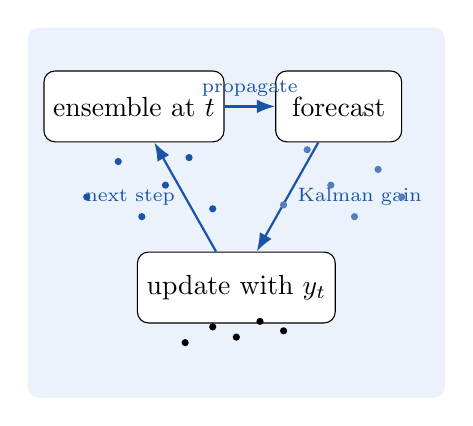
\begin{tikzpicture}[>=Latex, node distance=0.75cm]
  \fill[softblue,rounded corners] (-0.2,-0.35) rectangle (5.1,4.35);
  \node[draw,rounded corners,fill=white,minimum width=1.6cm,minimum height=0.9cm] (ens) at (1.15,3.35) {ensemble at $t$};
  \node[draw,rounded corners,fill=white,minimum width=1.6cm,minimum height=0.9cm] (pred) at (3.75,3.35) {forecast};
  \node[draw,rounded corners,fill=white,minimum width=1.6cm,minimum height=0.9cm] (upd) at (2.45,1.05) {update with $y_t$};
  \draw[->,thick,accent] (ens) -- node[above,font=\scriptsize] {propagate} (pred);
  \draw[->,thick,accent] (pred) -- node[right,font=\scriptsize] {Kalman gain} (upd);
  \draw[->,thick,accent] (upd) -- node[left,font=\scriptsize] {next step} (ens);
  \foreach \x/\y in {0.55/2.2,0.95/2.65,1.25/1.95,1.55/2.35,1.85/2.7,2.15/2.05} {
    \fill[accent] (\x,\y) circle (1.3pt);
  }
  \foreach \x/\y in {3.05/2.1,3.35/2.8,3.65/2.35,3.95/1.95,4.25/2.55,4.55/2.2} {
    \fill[accent!75] (\x,\y) circle (1.3pt);
  }
  \foreach \x/\y in {1.8/0.35,2.15/0.55,2.45/0.42,2.75/0.62,3.05/0.5} {
    \fill[black] (\x,\y) circle (1.3pt);
  }
\end{tikzpicture}
\end{columns}
\end{frame}

\begin{frame}{4. Problem Statement}
\begin{block}{Goal}
Given only noisy observations $\mathbf{y}_{1:T}$, we want to:
\begin{enumerate}
  \item infer the hidden states $\mathbf{x}_{1:T}$,
  \item learn the unknown nonlinear transition function $f$,
  \item keep uncertainty estimates for both.
\end{enumerate}
\end{block}

\vspace{1mm}
\begin{columns}[T,totalwidth=\textwidth]
\column{0.5\textwidth}
\begin{block}{Why this is hard}
\begin{itemize}
  \item Exact inference in GPSSM is \textbf{intractable}.
  \item Latent states and the GP transition are \textbf{strongly coupled}.
  \item The posterior is nonlinear and sequential.
\end{itemize}
\end{block}

\column{0.5\textwidth}
\begin{block}{Limitations of earlier approaches}
\begin{itemize}
  \item Mean-field approximations can be too crude.
  \item Richer variational families introduce many parameters.
  \item Inference networks may be unstable or expensive to train.
\end{itemize}
\end{block}
\end{columns}

\vspace{1mm}
\begin{center}
\Large \textbf{Need:} a tractable non-mean-field inference method for GPSSM.
\end{center}
\end{frame}

\begin{frame}{5. Proposed Solution: EnVI}
\begin{columns}[T,totalwidth=\textwidth]
\column{0.58\textwidth}
\begin{block}{Main idea}
Use a \textbf{sparse GP} for the transition model and use \textbf{EnKF} to \emph{implicitly} approximate the posterior over latent states.
\end{block}

\begin{itemize}
  \item Introduce inducing variables $\mathbf{u}$ for scalable GP inference.
  \item Do \textbf{not} parameterize the latent-state posterior directly.
  \item Instead, obtain filtering distributions from EnKF.
  \item Build an ELBO from:
  \begin{itemize}
    \item predictive log-likelihood terms,
    \item KL for the initial state,
    \item KL for GP inducing variables.
  \end{itemize}
  \item Optimize end-to-end with autodiff.
\end{itemize}

\column{0.42\textwidth}
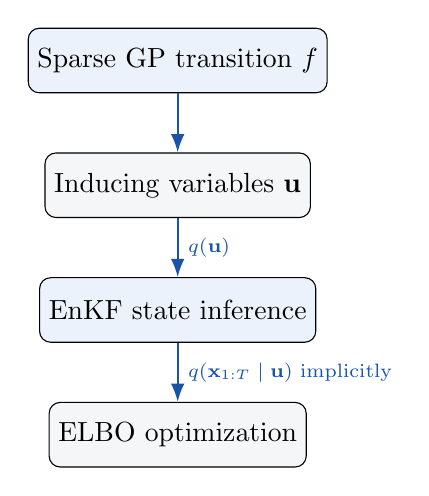
\begin{tikzpicture}[>=Latex, node distance=0.55cm]
  \node[draw,rounded corners,fill=softblue,minimum width=3.1cm,minimum height=0.82cm] (gp) {Sparse GP transition $f$};
  \node[draw,rounded corners,fill=softgray,minimum width=3.1cm,minimum height=0.82cm,below=0.75cm of gp] (u) {Inducing variables $\mathbf{u}$};
  \node[draw,rounded corners,fill=softblue,minimum width=3.1cm,minimum height=0.82cm,below=0.75cm of u] (enkf) {EnKF state inference};
  \node[draw,rounded corners,fill=softgray,minimum width=3.1cm,minimum height=0.82cm,below=0.75cm of enkf] (elbo) {ELBO optimization};
  \draw[->,thick,accent] (gp) -- (u);
  \draw[->,thick,accent] (u) -- node[right,font=\scriptsize] {$q(\mathbf{u})$} (enkf);
  \draw[->,thick,accent] (enkf) -- node[right,font=\scriptsize] {$q(\mathbf{x}_{1:T}\mid \mathbf{u})$ implicitly} (elbo);
  \node[align=center,font=\small] at (0.95,-0.25) {};
\end{tikzpicture}
\end{columns}

\vspace{1mm}
\begin{center}
\textbf{Interpretation:} GP learns the dynamics; EnKF tracks the latent trajectory; variational inference ties both together.
\end{center}
\end{frame}

\begin{frame}{6. Experiments}
\small
\begin{columns}[T,totalwidth=\textwidth]
\column{0.49\textwidth}
\begin{block}{Synthetic experiments}
\begin{itemize}
  \item \textbf{Linear Gaussian SSM:} EnVI recovers hidden states close to Kalman-filter quality.
  \item \textbf{Kink transition benchmark:} best MSE and log-likelihood across low / medium / high noise.
  \item Faster convergence than inference-network-based baselines.
\end{itemize}
\end{block}

\vspace{1mm}
\begin{tabular}{lccc}
\toprule
Noise & Low & Mid & High \\
\midrule
EnVI MSE & 0.0046 & 0.0536 & 0.5315 \\
\bottomrule
\end{tabular}

\column{0.51\textwidth}
\begin{block}{Real-world forecasting}
EnVI is best or highly competitive on standard benchmarks. It achieves the best RMSE on \textbf{4 of 5} datasets in the paper.
\end{block}

\vspace{1mm}
\begin{tabular}{lccccc}
\toprule
Dataset & Act. & Ball & Drive & Dryer & Gas \\
\midrule
EnVI & 0.657 & 0.055 & 0.703 & 0.125 & 1.388 \\
\bottomrule
\end{tabular}

\vspace{2mm}
\begin{itemize}
  \item Strong robustness across noise levels.
  \item Good latent-state inference and good forecasting accuracy.
\end{itemize}
\end{columns}
\end{frame}

\begin{frame}{7. Conclusion}
\begin{block}{Take-home message}
The paper shows how to combine:
\begin{itemize}
  \item \textbf{GP} for flexible probabilistic modeling of unknown dynamics,
  \item \textbf{GPSSM} for latent nonlinear dynamical systems,
  \item \textbf{EnKF} for efficient sequential state inference.
\end{itemize}
\end{block}

\vspace{1mm}
\begin{block}{Why the combination matters}
\begin{itemize}
  \item avoids an overly restrictive mean-field approximation,
  \item avoids heavy explicit parameterization of the latent posterior,
  \item yields a practical and differentiable inference algorithm,
  \item works well empirically on synthetic and real datasets.
\end{itemize}
\end{block}

\vspace{1mm}
\begin{center}
\normalsize \textbf{In one sentence:} EnVI uses EnKF as the latent-state inference engine\\[1mm]
inside variational learning of a sparse GPSSM.
\end{center}
\end{frame}

\end{document}

